A couple of neutral atoms interacting through Lennard-Jones potentials hardly 
feel each other as soon as they separate farther than three or four times 
$\sigma$, even if one of them is just the nearest of a huge cluster. Long-range 
interactions fall off much more slowly. The Earth feels the tug of the sun 
bending its trajectory from many millions of miles away. In the latter case, we 
cannot define a cut-off radius for interactions. In classical physics, the Earth 
will feel the attraction of other heavenly bodies no matter the distance. You 
cannot safely neglect their effect, as huge masses compensate for greater 
separations.

\section{Gravity}

You probably know that Newtonian gravitational forces obey an inverse-square
law, with the force of object $j$ on object $i$ given by
\begin{equation*}
  F(\mathrm{r}_{ij}) = G \frac{m_i m_j}{r_{ij}^2}\
                         \frac{\mathbf{r}_{ij}}{r_{ij}},
\end{equation*}
with $\mathbf{r}_{ij}$ standing for the vector going from $i$ to $j$, $m_i$ and
$m_j$ the masses, $r_{ij}$ the distance from $i$ to $j$, and $G$ the universal
gravitational constant.

A gravitational interaction would follow the same structure as the custom Morse 
potential that we wrote in section \ref{Custom_pair_potentials}, with a few 
differences. Apart from the obvious change in the functional form of the force 
and energy, the cut-off radius becomes infinite and the calculation of the 
forces and energies requires knowledge of the masses involved, so we have to 
include a \texttt{getInfo} function that provides them. The constructor will 
only receive the value of one parameter: the universal gravitational constant 
$G$. By now, you should find the whole following code block straightforward.
\begin{lstlisting}
%! codeblock: gravity
struct gravity {
  real G;

  gravity(real i_G) : G(i_G) {}

  real getCutOff() { return std::numeric_limits<real>::infinity(); }

  struct ForceEnergy {
    real4 * force;
    real * energy;
    real * mass;
    real G;

    ForceEnergy(real4 * i_force, real * i_energy,
                real * i_mass, real i_G):
                force(i_force), energy(i_energy),
                mass(i_mass), G(i_G){}

    __device__ real getInfo(int index) {
      return mass[index];
    }

    __device__ real4 compute(real4 ri, real4 rj, real mi, real mj){
      const real3 rij = make_real3(rj)-make_real3(ri);
      const real r2 = dot(rij, rij);
      const real r = sqrtf(r2);
      if(r2 > 0){
        return make_real4(G*(mi*mj/(r2*r))*rij,
                          -G*mi*mj/r);
      }
      return real4();
    }

    __device__ void set(int id, real4 total){
      force[id] += make_real4(total.x, total.y, total.z, 0);
      energy[id] += 0.5*total.w;
    }
  };

  ForceEnergy getForceEnergyTransverser(Box box,
                             std::shared_ptr<ParticleData> sys){
    auto force = sys->getForce(access::location::gpu,
                               access::mode::readwrite).raw();
    auto energy = sys->getEnergy(access::location::gpu,
                                 access::mode::readwrite).raw();
    auto mass = sys->getMass(access::location::gpu,
                             access::mode::read).raw();
    return ForceEnergy(force, energy, mass, G);
  }
};//!
%! codeblockend !//
\end{lstlisting}

For a realistic simulation of something like the solar system, you will have to 
read in the data from an external file. Let us agree that the file begins with 
an integer representing the number of objects contained in the file, followed by 
a row for each object listing the position coordinates, velocity vector, mass 
and name. Then you could set up the initial conditions with a block of code like 
this:
\begin{lstlisting}
%! codeblock: gravityInitialConditions
  auto sys = make_shared<System>(argc, argv);
  int numberOfParticles;

  std::ifstream in("solarSystem.dat");
  if(!std::ifstream("solarSystem.dat").good()) {
    sys->log<System::CRITICAL>("File solarSystem.dat not found.");
  }

  in>>numberOfParticles;

  auto particles
    = make_shared<ParticleData>(numberOfParticles, sys);

  {
    auto position
      = particles->getPos(access::location::cpu,
                          access::mode::write);
    auto velocity
      = particles->getVel(access::location::cpu,
                          access::mode::write);
    auto mass
      = particles->getMass(access::location::cpu,
                           access::mode::write);

    sys->log<System::MESSAGE>("Reading data for astronomical objects:");
    std::string objectName;

    for(int i = 0; i < numberOfParticles; ++i) {
      in>>position[i].x>>position[i].y>>position[i].z
        >>velocity[i].x>>velocity[i].y>>velocity[i].z
        >>mass[i]>>objectName;
      position[i].w = real(0.0);
      sys->log<System::MESSAGE>(objectName);
    }
  }//!
%! codeblockend !//
\end{lstlisting}

Work out the value of $G$ in your units of choice. For the solar system, I chose 
astronomical units, days and Earth masses. Then you can activate the interaction 
with the lines below. Figure \ref{gravity} shows some planetary trajectories 
resulting from my test simulation.
\begin{lstlisting}
%! codeblock: gravityInteractor
  real G = 8.888e-10;
  auto GPotential = make_shared<gravity>(G);
  {
    using GForces = PairForces<gravity>;

    auto interaction
      = make_shared<GForces>(particles, sys, GPotential);

    integrator->addInteractor(interaction);
  }//!
%! codeblockend !//
\end{lstlisting}

\begin{comment}
Integrating the code blocks into the gravity:
\begin{lstlisting}
%! codefile: code/gravity.cu
# include "uammd.cuh"
# include "utils/InitialConditions.cuh"
# include "Interactor/Potential/Potential.cuh"
# include "Interactor/NeighbourList/CellList.cuh"
# include "Interactor/PairForces.cuh"
# include "Integrator/VerletNVE.cuh"

using namespace uammd;
using std::make_shared;
using std::endl;

%! codeinsert: gravity

int main(int argc, char *argv[]){

  %! codeinsert: gravityInitialConditions

  using Verlet = VerletNVE;
  Verlet::Parameters VerletParams;
  VerletParams.dt = 0.01;
  VerletParams.initVelocities = false;

  auto integrator
    = make_shared<Verlet>(particles, sys, VerletParams);

  %! codeinsert: gravityInteractor

  std::string outputFile = "gravity.dat";
  std::ofstream out(outputFile);

  int numberOfSteps = 1000000;
  int printEverynSteps = 1000;

  for(int step = 0; step < numberOfSteps; ++step) {
    integrator->forwardTime();

    if(printEverynSteps > 0
       and step % printEverynSteps == 1) {
      auto position
        = particles->getPos(access::location::cpu,
                            access::mode::read);
      const int * index = particles->getIdOrderedIndices(access::location::cpu);

      out<<endl;
      for(int id = 0; id < numberOfParticles; ++id)
        out<<make_real3(position[index[id]])<<endl;
    }
  }

  sys->finish();

  return 0;
}//!
%! codeend !//
\end{lstlisting}
\end{comment}

\begin{figure}
  \begin{center}
  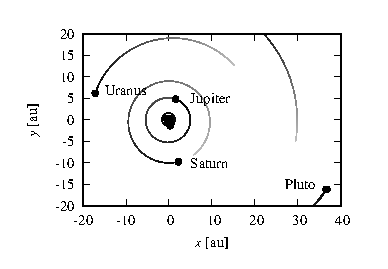
\includegraphics[width = 0.53\textwidth]{figures/gravity.eps}
  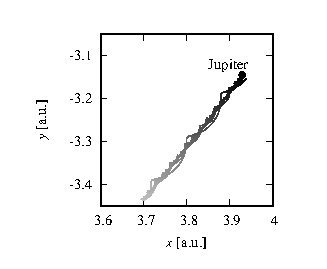
\includegraphics[width = 0.44\textwidth]{figures/Jupiter.eps}
  \end{center}
  \caption{\label{gravity}Motion of objects in the solar system for $10^4$ days 
           starting on the 10\textsuperscript{th} of March 2021, when the code 
           was run. In a close-up of a segment of the trajectory for Jupiter 
           (\textit{right}) you can also see the trajectories of some of its 
           moons (initial configuration data obtained from NASA JPL HORIZONS 
           system).}
\end{figure}

\section{Charge distributions}

The previous section might have given you the impression that the problem with 
long-range forces arises from having to consider all the pair interactions. In 
fact, fast multipole methods can speed up the calculations by cleverly grouping 
particles together, at the cost of a more complex algorithm. But, with the 
slower algorithm, our gravity simulator looks much like the Lennard-Jones 
simulator, only with infinite-range potentials. No big deal.

The real puzzle comes to light when you try to model something like charged 
atoms in a crystal, for here you would like to impose periodic boundary 
conditions. That means that a charge feels forces not just due to all the other 
charges you track, \textit{but also to the infinity of periodic images}.

To solve the problem, UAMMD employs the popular trick known as Ewald splitting. 
Instead of point charges, we use Gaussian distributions centered around the 
points and calculate the field as a sum of two contributions: one springing from 
the interaction with nearby atoms, the other a far field created by an infinite 
periodic distribution of charge. We have no need of concerning ourselves with 
the mathematical details here, as we will create an \texttt{interactor} much 
like any other in UAMMD, but you must remember that, if you wish to simulate a 
periodic distribution of charges, creating a new Coulomb pair potential would 
\textit{not} give you the right answer.

Before we write some more code, let me introduce you to a version of the 
Buckingham potential with an extra term tagging along.
\begin{equation*}
  V(r_{ij}) = A_{ij}e^{-B_{ij}r_{ij}} - \frac{C_{ij}}{r_{ij}^6}
                                      - \frac{D_{ij}}{r_{ij}^8}.
\end{equation*}
The distance $r_{ij}$ obviously refers to the separation between particles $i$ 
and $j$, but this time we have also added subindices to the parameters $A$, $B$, 
$C$ and $D$, because below we will consider two types of particles, sodium (Na) 
and chlorine (Cl) atoms, and the constants differ depending on the particles 
involved (as shown in Table \ref{NaCl_parameters}).

\begin{table}
    \begin{center}
      \begin{tabular}{| c | c | c | c | c |}
			\hline
      Interaction type & A (eV) & B (nm) & C ($10^{-6}$ eV nm$^6$) & D ($10^{-8}$ eV nm$^8$) \\
      \hline
      Na--Na           &    487 & 0.4208 &          1.05           &   0.499 \\
      Na--Cl           &  14514 & 0.4208 &          6.99           &   8.675 \\
      Cl--Cl           & 405774 & 0.4208 &         72.40           & 145.425 \\
      \hline
      \end{tabular}
    \end{center}
    \caption{\label{NaCl_parameters}Buckingham potential parameters for the 
             interactions of Na and Cl atoms (\textit{Source}: Q. Chen 
             \textit{et al.}, \textit{Molecular dynamics simulation of 
             thermodynamic properties of NaCl at high pressures and 
             temperatures}, Journal of Physics and Chemistry of Solids 
             \textbf{65} 1077--1081, 2004).}
\end{table}

In addition to this short-ranged potential, the atoms will feel the 
electrostatic interactions,
\begin{equation*}
  V_E(r_{ij}) = \frac{1}{4 \pi \epsilon_0} \frac{Z_i Z_j e^2}{r_{ij}},
\end{equation*}
but, as explained before, in a periodic setting.


\section{Hydrodynamics}

% Integrators

\section{Particle-based fluids}

\section{Lattice-Boltzmann}

\begin{comment}
List of programs written in this chapter:
%! codeblock: codelist
* `gravity.cu`: Simulation of astronomical bodies in the solar system.
%! codeblockend
\end{comment}
